\section{Overview of the MVAPICH Project}

InfiniBand, Omni-Path, Ethernet/iWARP and RDMA over 
Converged Ethernet (RoCE) are
emerging as high-performance networking technologies to deliver low latency and
high bandwidth.  They are also achieving widespread acceptance due to their {\em
open standards}.

MVAPICH (pronounced as ``em-vah-pich'') is an {\em open-source} MPI software to
exploit the novel features and mechanisms of these networking technologies and
deliver best performance and scalability to MPI applications.  This software is
developed in the \href{http://nowlab.cse.ohio-state.edu} {Network-Based
Computing Laboratory (NBCL)}, headed by
\href{http://www.cse.ohio-state.edu/~panda} {Prof. Dhabaleswar K. (DK) Panda}.

The MVAPICH2 MPI library supports MPI-3 semantics.  This {\em open-source} MPI
software project started in 2001 and a first high-performance implementation was
demonstrated at SuperComputing '02 conference.  After that, this software has
been steadily gaining acceptance in the HPC, InfiniBand, Omni-Path, 
Ethernet/iWARP and
RoCE communities. As of  May 2021, more than 3,150
organizations (National Labs, Universities and Industry) world-wide (in 89 
countries) have registered as MVAPICH users at MVAPICH project web site. There
have also been more than 1.36 million downloads of this 
software from the MVAPICH
project site directly.  In addition, many InfiniBand, Omni-Path, Ethernet/iWARP 
and 
RoCE vendors, server vendors, systems integrators and Linux distributors have
been incorporating MVAPICH2 into their software stacks and distributing it. 
%MVAPICH and MVAPICH2 are also available with the Open Fabrics Enterprise
%Distribution (OFED) stack. 
MVAPICH2 distribution is available under BSD licensing.

Several InfiniBand systems using MVAPICH2 have obtained positions in 
the TOP 500
ranking.  The Nov '20 list includes the following systems: 
4th, 10,649,600-core (Sunway TaihuLight) at National Supercomputing Center in
Wuxi, China
9th, 448, 448 cores (Frontera) at TACC
14th, 391,680 cores (ABCI) in Japan
21st, 570,020 cores (Neurion) in South Korea
22nd, 556,104 cores (Oakforest-PACS) in Japan
25th, 367,024 cores (Stampede2) at TACC
and 46th, 241,108-core (Pleiades) at NASA.
\%90, 76,032-core (Tsubame 2.5) at Tokyo Institute of Technology

More details on MVAPICH software, users list, mailing lists, sample performance
numbers on a wide range of platforms and interconnects, a set of OSU benchmarks,
related publications, and other InfiniBand-, RoCE, Omni-Path, and iWARP-related projects (High-Performance Big Data and High-Performance Deep Learning)
can be obtained from our
website:\href{http://mvapich.cse.ohio-state.edu}{http://mvapich.cse.ohio-state.edu}.


This document contains necessary information for MVAPICH2 users to download,
install, test, use, tune and troubleshoot MVAPICH2 \mvapichversion.  We
continuously fix bugs and update update this document as per user feedback.
Therefore, we strongly encourage you to refer to our web page for updates.
% As we get feedbacks from users and take care of bug-fixes, we introduce new
% tarballs and also continuously update this document.  Thus, we strongly
% request you to refer to our web page for updates.



\section{How to use this User Guide?}

This guide is designed to take the user through all the steps involved in
configuring, installing, running and tuning MPI applications over InfiniBand
using MVAPICH2 \mvapichversion.

In Section~\ref{sec:features} we describe all the features in MVAPICH2
\mvapichversion. As you read through this section, please note our new features
(highlighted as \textcolor{red}{NEW}) compared to version \mvapicholdversion.
Some of these features are designed in order to optimize specific type of MPI
applications and achieve greater scalability.  Section~\ref{sec:install}
describes in detail the configuration and installation steps.  This section
enables the user to identify specific compilation flags which can be used to
turn some of the features on or off.  Basic usage of MVAPICH2 is explained in
Section~\ref{sec:usage}. Section~\ref{sec:advanced_usage} provides instructions
for running MVAPICH2 with some of the advanced features.
Section~\ref{sec:osubenchmarks} describes the usage of the OSU Benchmarks.
In Section~\ref{sec:performance-tuning} we suggest some tuning techniques
for multi-thousand node clusters using some of our new features.  If you
have any problems using MVAPICH2, please check
Section~\ref{sec:troubleshooting} where we list some of the common
problems people face.  Finally, in Sections \ref{def:mvapich-parameters}
and \ref{def:mvapich-parameters-nem}, we list all important run time
parameters, their default values and a short description.



%---------------------------------------------------------

% \section{ MVAPICH2 \mvapichversion Modules }
% \label{sec:modules}
% 
% \begin{figure}[htbp]
%  \centering
%  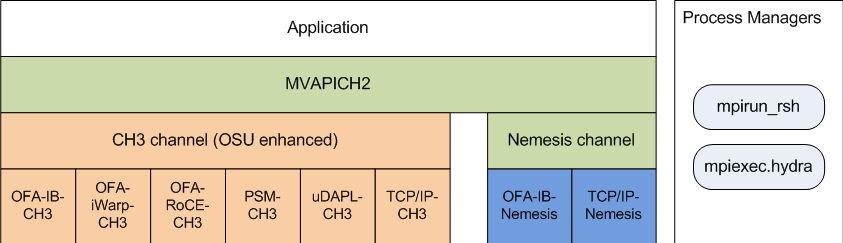
\includegraphics[width=0.6\textwidth]{modules-schema.png}
%  \caption{Schema of the modules of MVAPICH2.}
%  \label{fig:modules}
% \end{figure}
% 
% 
% \textbf{To be completed. Can be moved in sec. \ref{sec:features}?}

%---------------------------------------------------------

\section{MVAPICH2 \mvapichversion  Features }
\label{sec:features}

MVAPICH2 (MPI-3 over InfiniBand) is an MPI-3 implementation based on
\href{http://www.mpich.org/} {MPICH} ADI3 layer.  MVAPICH2 \mvapichversion is
available as a single integrated package (with MPICH \mpichversion).  The
current release supports ten different underlying transport interfaces, as shown
in Figure~\ref{fig:modules}. 
%In addition to the previous CH3-based interfaces, new interfaces based on
%MPICH2-Nemesis are introduced with this release.

\begin{figure}[htbp]
 \centering
 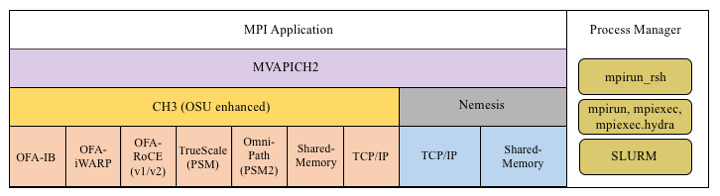
\includegraphics[width=0.9\textwidth]{Img/mv2-interfaces.png}
 \caption{Overview of different available interfaces of the MVAPICH2 library}
 \label{fig:modules}
\end{figure}

\begin{itemize}
\item{OFA-IB-CH3: This interface supports all InfiniBand
        compliant devices based on the 
        \href{http://www.openfabrics.org}
        {OpenFabrics} layer. This
        interface has the most features and is most widely used. For
        example, this interface can be used over all Mellanox InfiniBand
        adapters, IBM eHCA adapters and TrueScale adapters.}

\item{OFA-iWARP-CH3: This interface supports all iWARP
        compliant devices supported by OpenFabrics. For example, this
        layer supports Chelsio T3 adapters with the native iWARP mode.}

\item {OFA-RoCE-CH3: This interface supports the 
        emerging RoCE (RDMA over Converged Ethernet) interface 
        for Mellanox ConnectX-EN adapters with 10/40GigE switches.
        It provides support for RoCE v1 and v2.} 
 
\item{TrueScale (PSM-CH3): This interface provides native support for TrueScale
        adapters from Intel over PSM interface. 
        It provides high-performance point-to-point communication 
        for both one-sided and two-sided operations.}

\item{Omni-Path (PSM2-CH3): This interface provides native support for Omni-Path
        adapters from Intel over PSM2 interface. 
        It provides high-performance point-to-point communication 
        for both one-sided and two-sided operations.}

\item {Shared-Memory-CH3:
        This interface provides native shared
        memory support on multi-core platforms where communication is
        required only within a node. Such as SMP-only systems, laptops,
        etc.}

\item{TCP/IP-CH3: The standard TCP/IP 
        interface (provided by MPICH) to work
        with a range of network adapters supporting TCP/IP interface. 
        This interface can be used with IPoIB
        (TCP/IP over InfiniBand network) support of InfiniBand also.
        However, it will not deliver good performance/scalability as
        compared to the other interfaces.}

\item {TCP/IP-Nemesis: The standard TCP/IP 
        interface (provided by 
        MPICH Nemesis channel) 
        to work with a range of network adapters supporting TCP/IP interface. 
        This interface can be used with IPoIB (TCP/IP over 
        InfiniBand network) support of 
        InfiniBand also. However, it will not deliver good 
        performance/scalability as 
        compared to the other interfaces.}

\item {Shared-Memory-Nemesis: 
        This interface provides native shared
	memory support on multi-core platforms where communication is
	required only within a node. Such as SMP-only systems, laptops,
	etc.}

\item {\textcolor{red}{(DEPRECATED)} OFA-IB-Nemesis:
        This interface supports all 
        InfiniBand compliant devices based on the  
        OpenFabrics layer with the emerging Nemesis 
        channel of the MPICH stack. 
        This interface can be used by all Mellanox InfiniBand adapters.}

\end{itemize}

%The current release supports Gen2 verbs for InfiniBand. The implementation
%is based on Verbs Level Interface (Gen2), developed by the OpenIB group.
%MVAPICH2 also supports uDAPL (User Direct Access Programming Library) interface
%from release version 0.6.5 onward. This uDAPL support in MVAPICH2 provides
%portability across networks and platforms with highest performance.

%Please note that the support for VAPI interface has been deprecated
%since MVAPICH2
%1.2 because OpenFabrics interface is getting more popular. MVAPICH2 users still
%using VAPI interface are strongly requested to migrate to the OpenFabrics
%interface.

MVAPICH2 \mvapichversion is compliant with MPI 3 standard. In addition, MVAPICH2
\mvapichversion provides support and optimizations for NVIDIA GPU,
multi-threading and fault-tolerance (Checkpoint-restart,
Job-pause-migration-resume).  A complete set of features of MVAPICH2
\mvapichversion are indicated below. New features compared to v2.2
are indicated as \textcolor{red}{NEW}. 

\begin{itemize}
    \item \textcolor{red}{NEW} Based on and ABI compatible with MPICH-\mpichversion
  \item MPI-3 standard compliance
    \begin{itemize}
    \item Nonblocking collectives
    \item Neighborhood collectives
    \item MPI\_Comm\_split\_type support
    \item Support for MPI\_Type\_create\_hindexed\_block
    \item \textcolor{red}{NEW} Enhanced support for MPI\_T PVARs and CVARs
    \item \textcolor{red}{NEW} Enhanced performance for Allreduce, Reduce\_scatter\_block, Allgather, Allgatherv through new algorithms
    \item \textcolor{red}{NEW} Improved performance for small message collective operations
    \item \textcolor{red}{NEW} Improved performance of data transfers from/to non-contiguous buffers used by user-defined datatypes
    \item Nonblocking communicator duplication routine MPI\_Comm\_idup (will only work for single-threaded programs)
    \item MPI\_Comm\_create\_group support
    \item Support for matched probe functionality
    \item Support for "Const" (disabled by default)
    \end{itemize}
  \item  CH3-level design for scaling to multi-thousand cores with highest
  performance and reduced memory usage.
    \begin{itemize}
      \item    Support for MPI-3 RMA in OFA-IB-CH3, OFA-IWARP-CH3, OFA-RoCE-CH3, TrueScale (PSM-CH3) and Omni-Path (PSM2-CH3)
      \item  Support for Omni-Path architecture
      \begin{itemize}
        \item  Introduction of a new PSM2-CH3 channel for Omni-Path
      \end{itemize}
      \item  \textcolor{red}{NEW} Support for Marvel QEDR RoCE adapters
      \item  \textcolor{red}{NEW} Support for PMIx protocol for SLURM and JSM
      \item  \textcolor{red}{NEW} Support for RDMA\_CM based multicast group creation
      \item  Support for OpenPOWER architecture
      \item  \textcolor{red}{NEW} Support IBM POWER9 and POWER8 architecture
      \item  \textcolor{red}{NEW} Support Microsoft Azure HPC cloud platform
      \item  \textcolor{red}{NEW} Support Cavium ARM (ThunderX2) systems
      \item  \textcolor{red}{NEW} Support Intel Skylake architecture
      \item  \textcolor{red}{NEW} Support Intel Cascade Lake architecture
      \item  \textcolor{red}{NEW} Support AMD EPYC Rome architecture
          \begin{itemize}
          \item \textcolor{red}{NEW} Enhanced point-to-point and collective
              tuning for AMD ROME processor
          \end{itemize}
      \item  \textcolor{red}{NEW} Support for Broadcom NetXtreme RoCE HCA
          \begin{itemize}
          \item \textcolor{red}{NEW} Enhanced inter-node point-to-point for
              Broadcom NetXtreme RoCE HCA
          \end{itemize}
      \item  \textcolor{red}{NEW} Support architecture detection for Fujitsu A64fx processor
          \begin{itemize}
          \item \textcolor{red}{NEW} Enhanced point-to-point and collective
              tuning for Fujitsu A64fx processor
          \end{itemize}
	  \item \textcolor{red}{NEW} Support architecture detection for Oracle BM.HPC2 cloud shape
		  \begin{itemize}
		  \item \textcolor{red}{NEW}Enhanced point-to-point tuning for Oracle BM.HPC2 cloud shape
          \end{itemize}
      \item  \textcolor{red}{NEW} Support for Intel Knights Landing architecture
      \begin{itemize}
        \item \textcolor{red}{NEW} Efficient support for different Intel Knight's Landing (KNL) models
        \item Optimized inter-node and intra-node communication
        \item \textcolor{red}{NEW} Enhance large message intra-node performance with CH3-IB-Gen2 channel on Intel Knight's Landing
      \end{itemize}      
      \item  \textcolor{red}{NEW}  Support for executing MPI jobs in Singularity
      \item  Exposing several performance and control variables to MPI-3 Tools information interface (MPIT)
      \begin{itemize}
        \item  Enhanced PVAR support
        \item \textcolor{red}{NEW} Add multiple MPI\_T PVARs and CVARs for point-to-point and collective operations
      \end{itemize}
      \item  \textcolor{red}{NEW} Enhance performance of point-to-point
          operations for CH3-Gen2 (InfiniBand), CH3-PSM, and CH3-PSM2 (Omni-
          Path) channels
      \item  Enable support for multiple MPI initializations
      \item  Enhanced performance for small messages
      \item Flexibility to use internal communication buffers of different size
      \item  Enhanced performance for MPI\_Comm\_split through new bitonic algorithm
      \item  Tuning internal communication buffer size for performance
      \item Improve communication performance by removing locks from critical path
      \item Enhanced communication performance for small/medium message sizes
      \item  Reduced memory footprint
      \item  \textcolor{red}{NEW} Multi-rail support for UD-Hybrid channel
      \item  \textcolor{red}{NEW} Enhanced performance for UD-Hybrid code
      \item  Support for InfiniBand hardware UD-Multicast based collectives
      \item \textcolor{red}{NEW} Gracefully handle any number of HCAs
      \item  HugePage support
      \item  Integrated Hybrid (UD-RC/XRC) 
           design to get best performance on large-scale systems with 
           reduced/constant memory footprint 
      \item  Support for running with UD only mode
      \item  Support for MPI-2 Dynamic  
           Process Management on InfiniBand Clusters 
      \item  eXtended Reliable 
           Connection (XRC) support 
             \begin{itemize}
               \item  Enable XRC by default at configure time
             \end{itemize}
      \item  Multiple CQ-based design for Chelsio 
           10GigE/iWARP 
      \item  Multi-port support for 
           Chelsio 10GigE/iWARP
      \item  Enhanced iWARP design for 
           scalability to higher process count
      \item  Support iWARP interoperability between Intel NE020 and Chelsio T4 adapters
      \item  Support for 3D torus topology 
           with appropriate SL settings
      \item  Quality of Service (QoS) support with multiple InfiniBand SL 
      \item  \textcolor{red}{NEW}  Capability to run MPI jobs across multiple InfiniBand subnets
      \item   Enabling support for intra-node communications in RoCE mode without 
	  shared memory
      \item  On-demand Connection Management: This feature enables
      InfiniBand connections to be setup dynamically, enhancing the
      scalability of MVAPICH2 on clusters of thousands of nodes. 
        \begin{itemize}
          \item  Support for backing on-demand UD CM information 
          with shared memory for minimizing memory footprint
          \item  Improved on-demand
          InfiniBand connection setup
          \item  On-demand connection 
          management support with IB CM (RoCE Interface) 
	  \item  Native InfiniBand Unreliable Datagram (UD) based
	  asynchronous connection management for OpenFabrics-IB
	  interface. 
	  \item  RDMA CM based on-demand
	  connection management for OpenFabrics-IB and \\
	  OpenFabrics-iWARP interfaces. 
      \item  \textcolor{red}{NEW} Support to automatically detect IP address of IB/RoCE interfaces when RDMA CM is enabled without relying on mv2.conf file
	\end{itemize}
      

      \item  Message coalescing support
      to enable reduction of per Queue-pair send queues for reduction
      in memory requirement on large scale clusters. This design also
      increases the small message messaging rate
      significantly. Available for OFA-IB-CH3
      interface. 

%       \item  Hot-Spot Avoidance Mechanism
%       (HSAM) for alleviating network-congestion in large scale
%       clusters. Available for OFA-IB-CH3 interface. 

      \item  RDMA Read utilized for
      increased overlap of computation and communication for
      OpenFabrics device. Available for OFA-IB-CH3 and OFA-IB-iWARP-CH3
      interfaces. 

      \item  Shared Receive Queue (SRQ) with flow control. This design
      uses significantly less memory for MPI library. Available for
      OFA-IB-CH3 interface. 

      \item  Adaptive RDMA Fast Path with Polling Set for low-latency
      messaging. Available for OFA-IB-CH3 and OFA-iWARP-CH3
      interfaces. 

      \item  Header caching for low-latency

      \item  CH3 shared memory channel for 
      standalone hosts
      (including SMP-only systems and laptops) without any InfiniBand adapters
      
      \item  Unify process affinity support in OFA-IB-CH3, PSM-CH3 and PSM2-CH3 channels
      \item  Support to enable affinity with asynchronous progress thread
      \item  Allow processes to request MPI\_THREAD\_MULTIPLE when socket or NUMA node level affinity is specified
      \item   Reorganized HCA-aware process mapping
      \item   Dynamic identification of maximum read/atomic operations supported by HCA
      \item  Enhanced scalability for 
      RDMA-based direct one-sided communication
      with less communication resource. Available for 
      OFA-IB-CH3 and OFA-iWARP-CH3 
      interfaces.
      \item Removed libibumad dependency for building the library
      \item Option to disable signal handler setup
      \item Tuned thresholds for various architectures
      \item Option for selecting non-default gid-index in a loss-less fabric setup in RoCE mode
      \item Option to use IP address as a fallback if hostname cannot be resolved
      \item \textcolor{red}{NEW} Improved job-startup performance
      \item \textcolor{red}{NEW} Gracefully handle RDMA\_CM failures during job-startup
      \item Enhanced startup time for UD-Hybrid channel
      \item Provided a new runtime variable MV2\_HOMOGENEOUS\_CLUSTER for optimized startup on homogeneous clusters
      \item Improved debug messages and error reporting
      \item  Supporting large data transfers ($>$2GB)
      
    \end{itemize}
  

  \item Support for MPI communication from NVIDIA GPU device memory

   \begin{itemize}
      \item \textcolor{red}{NEW} Improved performance for Host buffers when CUDA
          is enabled
      \item \textcolor{red}{NEW} Add custom API to identify if MVAPICH2 has in-built CUDA support
      \item Support for MPI\_Scan and MPI\_Exscan collective operations from GPU buffers
      \item Multi-rail support for GPU communication
      \item Support for non-blocking streams in asynchronous CUDA transfers for better overlap
      \item Dynamic CUDA initialization. Support GPU device selection after MPI\_Init
      \item Support for running on heterogeneous clusters with GPU and non-GPU nodes
      \item Tunable CUDA kernels for vector datatype processing for GPU communication
      \item Optimized sub-array data-type processing for GPU-to-GPU communication
      \item Added options to specify CUDA library paths
      \item Efficient vector, hindexed datatype processing on GPU buffers
      \item Tuned MPI performance on Kepler GPUs
      \item Improved intra-node communication with GPU buffers using pipelined design
      \item Improved inter-node communication with GPU buffers with non-blocking CUDA copies
      \item Improved small message communication performance with CUDA IPC design
      \item Improved automatic GPU device selection and CUDA context management
      \item Optimal communication channel selection for different GPU communication 
           modes (DD, HH and HD) in different configurations (intra-IOH a and inter-IOH)
      \item Provided option to use CUDA library call instead of CUDA driver to check buffer pointer type
      \item  High performance RDMA-based 
           inter-node point-to-point 
           communication (GPU-GPU, GPU-Host and Host-GPU)

      \item  High performance intra-node point-to-point communication
           for multi-GPU adapters/node (GPU-GPU, GPU-Host and Host-GPU) 

      \item  Enhanced designs for Alltoall and Allgather collective 
           communication from GPU device buffers

      \item  Optimized and tuned support for collective communication from GPU buffers

      \item  Non-contiguous datatype support in point-to-point and collective
           communication from GPU buffers 
          
      \item  Updated to sm\_20 kernel optimizations for MPI Datatypes

      \item  Taking advantage of CUDA IPC (available in CUDA 4.1) in intra-node 
           communication for multiple GPU adapters/node

      \item  Efficient synchronization mechanism using CUDA Events for pipelined 
           device data transfers

    \end{itemize}


 %\item  Optimized support for nVIDIA GPU accelerators (with and without 
 %      GPUDirect technology)

\item  OFA-IB-Nemesis interface design  \textcolor{red}{(Deprecated)}
   \begin{itemize} 
      \item  OpenFabrics InfiniBand network module support for 
           MPICH Nemesis modular design    
      \item  Optimized adaptive RDMA fast path with Polling Set for high-performance
           inter-node communication
      \item  Shared Receive Queue (SRQ) support with flow control,
           uses significantly less memory for MPI library 
      \item  Header caching for low-latency
      \item  Support for additional features (such as hwloc, hierarchical 
           collectives, one-sided, multi-threading, etc.), as included 
           in the MPICH Nemesis channel
      \item  Support of Shared-Memory-Nemesis interface 
	   on multi-core platforms  requiring intra-node communication only 
	   (SMP-only systems, laptops,  etc.)
      \item  Support for 3D torus topology 
           with appropriate SL settings
      \item  Quality of Service (QoS) support with multiple InfiniBand SL 
      \item  Automatic inter-node communication parameter tuning based on platform and adapter detection
      \item  Flexible HCA selection 
      \item  Checkpoint-Restart support
      \item  Run-through stabilization support to handle process failures 
      \item  Enhancements to handle IB errors gracefully 
    
  \end{itemize}
  \item  Flexible process manager support
     \begin{itemize}
      \item Support for PMI-2 based startup with SLURM
      \item  Enhanced startup performance with SLURM
        \begin{itemize}
            \item  Support for PMIX\_Iallgather and PMIX\_Ifence
        \end{itemize}
         \item   Enhanced startup performance and reduced memory
            footprint for storing InfiniBand end-point information with SLURM
        \begin{itemize}
            \item  Support for shared memory based PMI operations
        \end{itemize}
      \item  \textcolor{red}{NEW}  On-demand connection management for PSM-CH3 and PSM2-CH3 channels
      \item  \textcolor{red}{NEW}  Support for JSM and Flux resource managers
      \item  \textcolor{red}{NEW} Enhanced job-startup performance for flux job launcher
      \item  \textcolor{red}{NEW} Improved job startup performance with mpirun\_rsh
	  \item  \textcolor{red}{NEW} Support in mpirun\_rsh for using srun daemons to launch jobs
      \item  \textcolor{red}{NEW} Support in mpirun\_rsh for specifying processes per node using '-ppn'
      \item  Improved startup performance for TrueScale (PSM-CH3) channel
      \item  \textcolor{red}{NEW} Improved job startup time for OFA-IB-CH3, PSM-CH3, and PSM2-CH3
      \item  Improved hierarchical job startup performance
       \item  Enhanced hierarchical ssh-based robust mpirun\_rsh framework 
       to work with any interface (CH3 and Nemesis channel-based) including OFA-IB-Nemesis, 
       TCP/IP-CH3 and TCP/IP-Nemesis to launch jobs on multi-thousand core clusters
       \item  Introduced option to export environment variables automatically with mpirun\_rsh
       \item  Support for automatic detection of path to utilities(rsh, ssh, xterm, TotalView)
                used by mpirun\_rsh during configuration
       \item  Support for launching jobs on heterogeneous networks with mpirun\_rsh
       \item  MPMD job launch capability 
       \item  Hydra process manager to work with any 
        of the ten interfaces (CH3 and 
       Nemesis channel-based) including OFA-IB-CH3, OFA-iWARP-CH3, 
       OFA-RoCE-CH3 and TCP/IP-CH3
       \item  Improved debug message output in process management and fault tolerance functionality
       \item  Better handling of process signals and error management in mpispawn

       \item  Flexibility for process execution with alternate group IDs
       \item  Using in-band IB communication with MPD
       \item  SLURM integration with mpiexec.mpirun\_rsh to use SLURM allocated
            hosts without specifying a hostfile
       \item  Support added to automatically use PBS\_NODEFILE in Torque and PBS
            environments
       \item  Support for suspend/resume functionality with mpirun\_rsh framework 
       \item  Exporting local rank, local size, 
            global rank and global size through environment variables (both mpirun\_rsh and hydra)
     \end{itemize}

  \item  Support for various job launchers and job schedulers 
(such as SGE and OpenPBS/Torque)

  \item  Configuration file support 
      (similar to one available in MVAPICH). Provides a convenient 
      method for handling all runtime variables through a configuration
      file. 
 
  \item 
    Fault-tolerance support
    \begin{itemize}
      \item Checkpoint-Restart Support with DMTCP (Distributed MultiThreaded CheckPointing)
      \item Enable hierarchical SSH-based startup with Checkpoint-Restart
      \item Enable the use of Hydra launcher with
		Checkpoint-Restart for OFA-IB-CH3 and OFA-IB-Nemesis interfaces
      \item  Checkpoint/Restart using LLNL's Scalable Checkpoint/Restart Library (SCR)
        \begin{itemize}
        \item  Support for application-level checkpointing
        \item  Support for hierarchical system-level checkpointing
        \end{itemize}
      \item  Checkpoint-restart support for application transparent
      systems-level fault tolerance. 
      \href{http://ftg.lbl.gov/CheckpointRestart/CheckpointRestart.shtml}{BLCR-based} 
      support using OFA-IB-CH3 and OFA-IB-Nemesis interfaces
        \begin{itemize}
          \item  Scalable Checkpoint-restart with 
               mpirun\_rsh framework 
          \item  Checkpoint-restart with
                 \href{http://www.mcs.anl.gov/research/cifts/index.php}{
                   Fault-Tolerance Backplane (FTB)} framework (FTB-CR)
          \item  Checkpoint-restart with 
               intra-node shared memory (user-level) support
          \item  Checkpoint-restart with 
               intra-node shared memory (kernel-level with LiMIC2) support
          \item  Checkpoint-restart 
               support with pure SMP mode 
          \item  Allows best performance and scalability with fault-tolerance
               support
          \item  Run-through stabilization support to handle process failures using OFA-IB-Nemesis interface
          \item  Enhancements to handle IB errors gracefully using OFA-IB-Nemesis interface
        \end{itemize}
      \item  Application-initiated system-level checkpointing is
      also supported. User application can request a whole program
      checkpoint synchronously by calling special MVAPICH2 functions.
        \begin{itemize} \item  Flexible interface to work with different files
	systems. Tested with ext3 (local disk), NFS and PVFS2. 
	\end{itemize}
      \item  Network-Level fault tolerance with Automatic Path
      Migration (APM) for tolerating intermittent network failures
      over InfiniBand. 
      \item  Fast Checkpoint-Restart support with aggregation scheme
      \item  Job Pause-Migration-Restart Framework for Pro-active Fault-Tolerance
           \begin{itemize}
            \item  Enable signal-triggered (SIGUSR2) migration
           \end{itemize}
      \item  Fast process migration using RDMA
      \item  Support for new standardized Fault Tolerant Backplane (FTB) Events
	   for Checkpoint-Restart and Job Pause-Migration-Restart Framework
    \end{itemize}
  \item  Enhancement to software installation
      \begin{itemize}  
        \item Revamped Build system
        \begin {itemize}
            \item  Uses automake instead of simplemake,
            \item  Allows for parallel builds ("make -j8" and similar)
        \end{itemize}
       \item  Full autoconf-based configuration
       \item  Automatically
      detects system architecture and adapter types and
      optimizes MVAPICH2 for any particular installation.
       \item  A utility (mpiname) for querying the MVAPICH2 
            library version and configuration information
	    \item  Automatically builds and installs OSU Benchmarks for end-user convenience
      \end{itemize}
  \item 
    Optimized intra-node communication support by taking advantage of
    shared-memory communication.  Available for all interfaces 
    (IB and iWARP).  
    \begin{itemize}
      \item \textcolor{red}{NEW}  Improve support for large processes per node
          and hugepages on SMP systems
      \item  Enhanced intra-node SMP performance
      \item  Tuned SMP eager threshold parameters
      \item  New shared memory design for enhanced intra-node small message performance
      \item  \textcolor{red}{NEW} Enhanced performance for shared-memory collectives
      \item  Support for single copy intra-node communication using Linux supported CMA (Cross Memory Attach)
          \begin{itemize}
            \item  Enabled by default
	    \item \textcolor{red}{NEW} Give preference to CMA if LiMIC2 and CMA are enabled at the same time
          \end{itemize}
      \item  Kernel-level single-copy 
           intra-node communication solution based on LiMIC2
           \begin{itemize}
            \item  Upgraded to LiMIC2 version 0.5.6 to support unlocked ioctl calls
            \item  LiMIC2 is designed and developed by jointly by The Ohio State University and System Software Laboratory at Konkuk University, Korea.
           \end{itemize}
      \item  Efficient Buffer Organization for Memory Scalability of 
           Intra-node Communication 
      \item  Multi-core optimized
      \item  Adjust shared-memory communication block size at runtime
      \item \textcolor{red}{NEW} Enhanced intra-node and inter-node tuning for PSM-CH3 and PSM2-CH3 channels
      \item \textcolor{red}{NEW} Added logic to detect heterogeneous CPU/HFI configurations in PSM-CH3 and PSM2-CH3 channels
      \item \textcolor{red}{NEW} support for process placement aware HCA
          selection
      \item  Automatic intra-node communication parameter tuning based on platform
      \item  Efficient connection set-up for multi-core systems
      \item  \textcolor{red}{NEW}  Portable Hardware Locality (hwloc v\hwlocvOneVersion)
           support for defining CPU affinity 
      \item  \textcolor{red}{NEW}  Portable Hardware Locality (hwloc v\hwlocvTwoVersion)
           support for defining CPU affinity 
      \item  \textcolor{red}{NEW}  NUMA-aware hybrid binding policy for dense
numa systems such as AMD EPYC (hwloc v\hwlocvOneVersion)
      \item  \textcolor{red}{NEW} NUMA-aware hybrid binding policy for dense
numa systems such as AMD EPYC (hwloc v\hwlocvTwoVersion)
      \item   \textcolor{red}{NEW} Add support to select hwloc v1 and hwloc v2
          at configure time
      \item  \textcolor{red}{NEW} Efficient CPU binding policies
           (spread, bunch, and scatter) to specify CPU binding per job for 
           modern multi-core platforms with SMT support
      \item  \textcolor{red}{NEW} Improved multi-rail selection logic
      \item  \textcolor{red}{NEW} Improved heterogeneity detection logic for HCA
and CPU
      \item  Enhanced support for CPU binding with socket and numanode level granularity
      \item  Enhance MV2\_SHOW\_CPU\_BINDING to enable display of CPU bindings on all nodes
      \item Improve performance of architecture detection
      \item Enhanced process mapping support for multi-threaded MPI applications
          \begin{itemize}
              \item \textcolor{red}{NEW} Improve support for process to core
                  mapping on many-core systems
              \begin{itemize}
              \item New environment variable MV2\_HYBRID\_BINDING\_POLICY for
                  multi-threaded MPI and MPI+OpenMP applications
              \item Support `spread', `linear', and `compact' placement of
                  threads
              \item Warn user if oversubcription of core is detected
              \end{itemize}
              \item  \textcolor{red}{NEW}  Introduce MV2\_CPU\_BINDING\_POLICY=hybrid 
              \item  \textcolor{red}{NEW}  Introduce MV2\_HYBRID\_BINDING\_POLICY
              \item  \textcolor{red}{NEW}  Introduce MV2\_THREADS\_PER\_PROCESS 
          \end{itemize}

      \item  Improved usability of process to CPU mapping with support of delimiters (',' , '-') in CPU listing
      \item  Also allows user-defined CPU binding 
      \item  Optimized for Bus-based SMP and NUMA-Based SMP systems. 
      \item  Efficient support for diskless clusters 
       
    \end{itemize}
  
  
  \item 
    Optimized collective communication
    operations. Available for OFA-IB-CH3, OFA-iWARP-CH3, and  OFA-RoCE-CH3 interfaces
    \begin{itemize}
        \item  \textcolor{red}{NEW}  Enhanced small message performance for Alltoallv
        \item  \textcolor{red}{NEW}  Support collective offload using Mellanox's
            SHARP for Allreduce and Barrier 
        \item \textcolor{red}{NEW}  Support collective offload using Mellanox's
            SHARP for Reduce and Bcast
        \item \textcolor{red}{NEW}  Enhanced tuning framework for Reduce and Bcast using SHARP
        \item  \textcolor{red}{NEW}  Enhanced collective tuning for OpenPOWER
(POWER8 and POWER9), Intel Skylake and Cavium ARM (ThunderX) systems
	\item  \textcolor{red}{NEW} Enhanced point-to-point and collective tuning
        for AMD EPYC Rome, Frontera@TACC, Longhorn@TACC, Mayer@Sandia,
        Pitzer@OSC, Catalyst@EPCC, Summit@ORNL, Lassen@LLNL, Sierra@LLNL,
        Expanse@SDSC, Ookami@StonyBrook, and bb5@EPFL systems
        \item  \textcolor{red}{NEW}  Enhanced collective tuning for Intel Knights Landing and Intel Omni-path
        \item  \textcolor{red}{NEW}  Enhance collective tuning for Bebop@ANL,
            Bridges@PSC, and Stampede2@TACC systems
        \item \textcolor{red}{NEW} Efficient CPU binding policies
      \item  Optimized collectives (bcast, reduce, and allreduce) for 4K processes
      \item  Optimized and tuned blocking and non-blocking collectives for OFA-IB-CH3, OFA-IB-Nemesis and TrueScale (PSM-CH3) channels
      \item  Enhanced MPI\_Bcast, MPI\_Reduce, MPI\_Scatter, MPI\_Gather performance
      \item  Hardware UD-Multicast based designs for collectives - Bcast, Allreduce and Scatter
      \item  Intra-node Zero-Copy designs for MPI\_Gather collective (using LiMIC2)
      \item  Enhancements and optimizations for point-to-point designs for Broadcast, Allreduce collectives
      \item  Improved performance for shared-memory based collectives - Broadcast, Barrier, Allreduce, Reduce
      \item  Performance improvements in Scatterv and Gatherv collectives for CH3 interface
      \item  Enhancements and optimizations for collectives (Alltoallv, Allgather)
      \item  Tuned Bcast, alltoall, Scatter, Allgather, Allgatherv, Reduce, Reduce\_Scatter, Allreduce collectives
    \end{itemize}
  

  \item 
    Integrated multi-rail communication support. Available for
    OFA-IB-CH3 and OFA-iWARP-CH3 interfaces.
    \begin{itemize}
        \item  Supports multiple queue pairs per port and 
             multiple ports per adapter 
	\item  Supports multiple adapters 
        \item  Support to selectively use 
             some or
             all rails according to user specification
	\item  Support for both one-sided and point-to-point operations 
        \item  Reduced stack size of internal threads to dramatically reduce 
	      memory requirement on multi-rail
        systems
	\item  Dynamic detection of multiple InfiniBand adapters 
	     and using these by default in multi-rail configurations (OFA-IB-CH3, OFA-iWARP-CH3 and OFA-RoCE-CH3 interfaces)
	\item  Support for process-to-rail binding policy (bunch, scatter and  user-defined) 
	     in multi-rail configurations (OFA-IB-CH3, OFA-iWARP-CH3 and OFA-RoCE-CH3 interfaces)
    \item  \textcolor{red}{NEW} Enhance HCA detection to handle cases where node has both IB and RoCE HCAs
    \item  \textcolor{red}{NEW} Add support to auto-detect RoCE HCAs and
        auto-detect GID index
    \item  \textcolor{red}{NEW} Add support to use RoCE/Ethernet and InfiniBand
        HCAs at the same time
    \end{itemize}
  

  \item  Support for InfiniBand Quality of Service (QoS) with multiple lanes

  \item 
    Multi-threading support. Available for all interfaces (IB and iWARP),
    including TCP/IP.
    \begin{itemize}
      \item  Enhanced support for multi-threaded applications
      \item \textcolor{red}{NEW}  Add support to enable fork safety in MVAPICH2 using environment variable
    \end{itemize}
  

  \item  
    High-performance optimized and scalable support for one-sided
    communication: Put, Get and Accumulate. Supported synchronization
    calls: Fence, Active Target, Passive (lock and unlock). Available
	for all interfaces.
	\begin{itemize}
          \item  Support for handling very large messages in RMA
          \item  Enhanced direct RDMA based designs for MPI\_Put and MPI\_Get operations in OFA-IB-CH3 channel
          \item  Optimized communication when using MPI\_Win\_allocate for OFA-IB-CH3 channel
          \item  Direct RDMA based One-sided communication support for OpenFabrics
	       Gen2-iWARP and RDMA CM (with Gen2-IB)
          \item  Shared memory backed Windows 
               for one-sided communication 
  	 
	\end{itemize}
  

  \item 
    Two modes of communication progress
    \begin{itemize}
      \item  Polling 
      \item  Blocking (enables running multiple MPI
      processes/processor). Available for OpenFabrics (IB and iWARP)
      interfaces. 
    \end{itemize}
  


  \item  Advanced AVL tree-based Resource-aware registration cache 
  \item  Adaptive number of registration cache entries based on job size
  
  \item  Automatic detection and tuning for 24-core Haswell architecture
  \item  Automatic detection and tuning for 28-core Broadwell architecture
  \item  Automatic detection and tuning for Intel Knights Landing architecture

  \item  Automatic tuning based on both platform type and network adapter

  \item    Remove verbs dependency when building the PSM-CH3 and PSM2-CH3 channels
  \item  Progress engine optimization for TrueScale (PSM-CH3) interface

  \item  Improved performance for medium size messages for TrueScale (PSM-CH3) channel

  \item  Multi-core-aware collective support for TrueScale (PSM-CH3) channel

  \item  Collective optimization for TrueScale (PSM-CH3) channel

  \item  Memory Hook Support provided by integration with ptmalloc2
  library. This provides safe release of memory to the Operating
  System and is expected to benefit the memory usage of applications
  that heavily use malloc and free operations. 

  \item  Warn and continue when ptmalloc fails to initialize
  \item \textcolor{red}{NEW} Add support to intercept aligned\_alloc in ptmalloc

  \item  Support for TotalView debugger with mpirun\_rsh framework  

  \item \textcolor{red}{NEW} Remove dependency on underlying libibverbs,
      libibmad, libibumad, and librdmacm libraries using dlopen

  \item  Support for linking Intel Trace Analyzer and Collector

  \item  Shared library support for existing binary MPI application 
       programs to run. 
   \item  Enhanced debugging config options to generate core files and back-traces
   \item  Use of gfortran as the default F77 compiler 
   \item \textcolor{red}{NEW}  Add support for MPI\_REAL16 based reduction opertaions for Fortran programs 
   \item  \textcolor{red}{NEW} Supports AMD Optimizing C/C++ (AOCC) compiler v2.1.0 
   \item  \textcolor{red}{NEW} Enhanced support for SHArP v2.1.0

  \item  ROMIO Support for MPI-IO. 
      \begin{itemize}
       \item  \textcolor{red}{NEW} Support for DDN Infinite Memory Engine (IME)
       \item  Optimized, high-performance ADIO driver for Lustre
      \end{itemize}

  \item  Single code base for the following platforms (Architecture, OS,
  Compilers, Devices and InfiniBand adapters)
    \begin{itemize}
      \item   Architecture: Knights Landing, OpenPOWER(POWER8 and POWER9), ARM, EM64T, x86\_64 and x86
      \item  Operating Systems: (tested with) Linux 
      \item  Compilers: GCC, Intel, PGI, and Open64
		  \begin{itemize}
		  \item \textcolor{red}{NEW} Support for GCC compiler v11
		  \item \textcolor{red}{NEW} Support for Intel IFX Compiler
		  \end{itemize}
      \item   Devices: OFA-IB-CH3, OFA-iWARP-CH3, OFA-RoCE-CH3, TrueScale (PSM-CH3), 
             Omni-Path (PSM2-CH3), TCP/IP-CH3, OFA-IB-Nemesis and TCP/IP-Nemesis 
      \item  InfiniBand adapters (tested with):
        \begin{itemize} 
          \item  Mellanox InfiniHost adapters (SDR and DDR) 
          \item  Mellanox ConnectX (DDR and QDR with PCIe2)
          \item  Mellanox ConnectX-2 (QDR with PCIe2)
          \item  Mellanox ConnectX-3 (FDR with PCIe3)
          \item  Mellanox Connect-IB (Dual FDR ports with PCIe3)
          \item  Mellanox Connect-4 (EDR with PCIe3)
          \item  Mellanox ConnectX-5 (EDR with PCIe3)
          \item  Mellanox ConnectX-6 (HDR with PCIe3)
	      \item  Intel TrueScale adapter (SDR) 
	      \item  Intel TrueScale adapter (DDR and QDR with PCIe2)
	    \end{itemize}
      \item  Intel Omni-Path adapters (tested with):
        \begin{itemize} 
	      \item  Intel Omni-Path adapter (100 Gbps with PCIe3)
	    \end{itemize}
      
      \item  10GigE (iWARP and RoCE) adapters:
        \begin{itemize} \item  (tested with) Chelsio T3 and T4 adapter with iWARP support  
%	  \item  Support for Chelsio's T4 adapter
          \item  (tested with) Mellanox ConnectX-EN 10GigE adapter 
          \item  (tested with) Intel NE020 adapter with iWARP support 
        \end{itemize}
      
      \item  40GigE RoCE adapters:
        \begin{itemize}
          \item  (tested with) Mellanox ConnectX-EN 40GigE adapter 
        \end{itemize}
    \end{itemize}
  

\end{itemize}

The MVAPICH2 \mvapichversion package and the project also includes the following provisions:

\begin{itemize}
        {\item
        \href{https://scm.nowlab.cse.ohio-state.edu/svn/mpi/mvapich2/} {Public SVN} access of the code-base}
    {\item A set of micro-benchmarks (including multi-threading latency test)
    for carrying out MPI-level performance evaluation after the installation}
    {\item Public \href{http://mailman.cse.ohio-state.edu/mailman/listinfo/mvapich-discuss} {mvapich-discuss} mailing list for mvapich users to
    \begin{itemize}
            {\item Ask for help and support from each other and get prompt response}
        {\item Enable users and developers to contribute patches and enhancements}
    \end{itemize}
    }
\end{itemize}
